\section{Introduction}
Le modèle Destinie 2 (modèle Démographique Économique et Social de Trajectoires INdividuelles sImulÉs, version 2) est un modèle de microsimulation dynamique, développé et géré par l'Insee, dont l'objectif principal est la projection à long terme des retraites.\\

La simulation se fait au niveau individuel, sur la base d'un échantillon représentatif de la population française au 1er janvier 2010. Cet échantillon est construit à partir de l'enquête Patrimoine 2009-2010 et est composé de 62 000 individus. Le modèle projette les situations familiales, carrières professionnelles et départs à la retraite des personnes de cette population, dont le renouvellement est assuré par la simulation des naissances, décès et flux migratoires. Les individus sont répartis en trois grands groupes : les salariés du secteur privé, les titulaires de la fonction publique et les indépendants. Il s'agit donc d'un modèle simplifié : par exemple, les membres des régimes spéciaux sont considérés comme affiliés au secteur privé ou aux titulaires de la fonction publique. Au niveau d’un individu, Destinie 2 permet de suivre l’ensemble de sa trajectoire professionnelle (statuts d’activité et revenus), et simule les liquidations à la retraite sous diverses hypothèses de comportement et de législation. Les liens familiaux (unions, naissances, séparations) étant également simulés, ce modèle permet également de réaliser des estimations au niveau du ménage.\\

Le modèle comprend deux modules distincts : le module générateur de biographies et le module de simulation des droits retraite.\\
La constitution des biographies démographiques s'appuie sur les dernières projections démographiques de l'Insee, couvrant la période 2013-2070 et le champ France entière. Les trajectoires professionnelles des individus sont connues jusqu’en 2009, année de base. \`A compter de 2010, leurs carrières (statuts d’activité et revenus) sont projetées en respectant des contraintes de calage sur des hypothèses macroéconomiques. Ces hypothèses portent sur la croissance de la productivité du travail et le taux de chômage, fournis par le Conseil d'Orientation des Retraites (COR), et le taux d'activité, repris des projections de population active de l'Insee.\\
Le module retraite simule le départ à la retraite selon la date de législation et l'hypothèse de comportement de liquidation choisies, et calcule le montant des droits associés. Les droits couvrent la pension de droit direct et de réversion des régimes de base (le régime général, le Service des Retraites de l'État (SRE) et la Caisse nationale de retraites des agents des collectivités locales (CNRACL), la Sécurité Sociale pour les Indépendants (SSI)) et complémentaires (Association pour le régime de retraite complémentaire des salariés(Arrco), Association générale des institutions de retraite complémentaire des cadres(Agirc)). La dimension ménage permet aussi d'inclure le minimum vieillesse.\\
Ce document détaille le contenu des fichiers de code source du modèle. 



\section{Vue d'ensemble}

Le programme est un package R écrit en C++. Il peut
être directement utilisé à partir d'une console en R, 
pour effectuer des simulations en fonction d'un échantillon
directement importable en R, et en passant les paramètres de la simulation
toujours depuis R. En revanche, le package en lui-même est écrit en C++. 

Structure des répertoires du package :

	\begin{description}
		\item[src] contient les fichiers sources du package écrits en C++
		\item[R] contient les fichiers sources du package écrits en R
		\item[parametres] contient les paramètres démographiques et macroéconomiques utilisés lors de la projection\\
Le sous-répertoire {\tt Projections\_COR\_2018} comprend les 5 scénarios économiques du rapport de juin 2018 du COR (voir la table \ref{tab:hypscCOR}). 
\renewcommand{\arraystretch}{1.8}
\newcolumntype{C}{>{\centering\arraybackslash}X}

\begin{table}[h]
  \centering
  \caption{Scénarios économiques du COR}
    \begin{tabular}{rr}
    \toprule
 Croissance du SMPT & Taux de chômage \\
    \midrule
 1,8     & 4,5 \\
 1,8   & 7 \\
 1,5   & 7 \\
 1,3   & 7 \\
 1     & 7 \\
 1     & 10 \\
    \bottomrule
    \end{tabular}%
  \label{tab:hypscCOR}%
\end{table}%
		\item[test] contient un échantillon test \textbf{non représentatif} de la population mais que l'on peut utiliser pour prendre en main le modèle de microsimulation
		\item[documentation] contient la documentation du package, des conseils pratiques, la liste des documents de travail de l'Insee publiés à partir du modèle Destinie 2 et la liste des contributeurs du modèle.
	\end{description}






\subsection{Le package Destinie}


Le programme est structuré autour de cinq classes d'objets et de structures (voir la figure \ref{fig:structGenePack}).\\
\begin{description}
\item[La classe Simulation] contient l'ensemble des paramètres d'une simulation ainsi que 
l'échantillon issu du générateur de biographies
utilisé sous la forme d'un tableau d'objets Indiv.
\item[La classe Indiv] contient l'ensemble des informations relatives à un individu donné.
\item[La classe Retraite] contient les variables sur les pensions (de droit direct ou dérivé) 
pour un individu et une année donnés.
\item[La classe DroitsRetr] contient l'ensemble des variables concernant la liquidation des
droits directs.
\item[La classe Legislation] contient l'ensemble des paramètres législatifs pour une date de législation, une année et un individu donnés. 
\item[La structure Macro] contient l'ensemble des paramètres macroéconomiques (PIB, inflation,...) mais aussi des 
paramètres plus spécifiques aux retraites (taux de cotisation, valeur des points dans les complémentaires ou encore montant du minimum vieillesse).
\end{description}

De plus, les fichiers {\tt Demographie.cpp}  et {\tt Destinie.h} contiennent les fonctions qui peuvent être appelées directement depuis R,
ainsi que les constantes du modèles.
Le fichier {\tt OutilsBase.h} contient également des fonctions utilitaires.\\

Le fichier simulation.R donne enfin un exemple de lancement de la simulation.



\phantom{sdfgsdgf
sdfgsdg}

\medskip 

\begin{landscape}
\begin{figure}
\caption{Structure générale du package}
\label{fig:structGenePack}
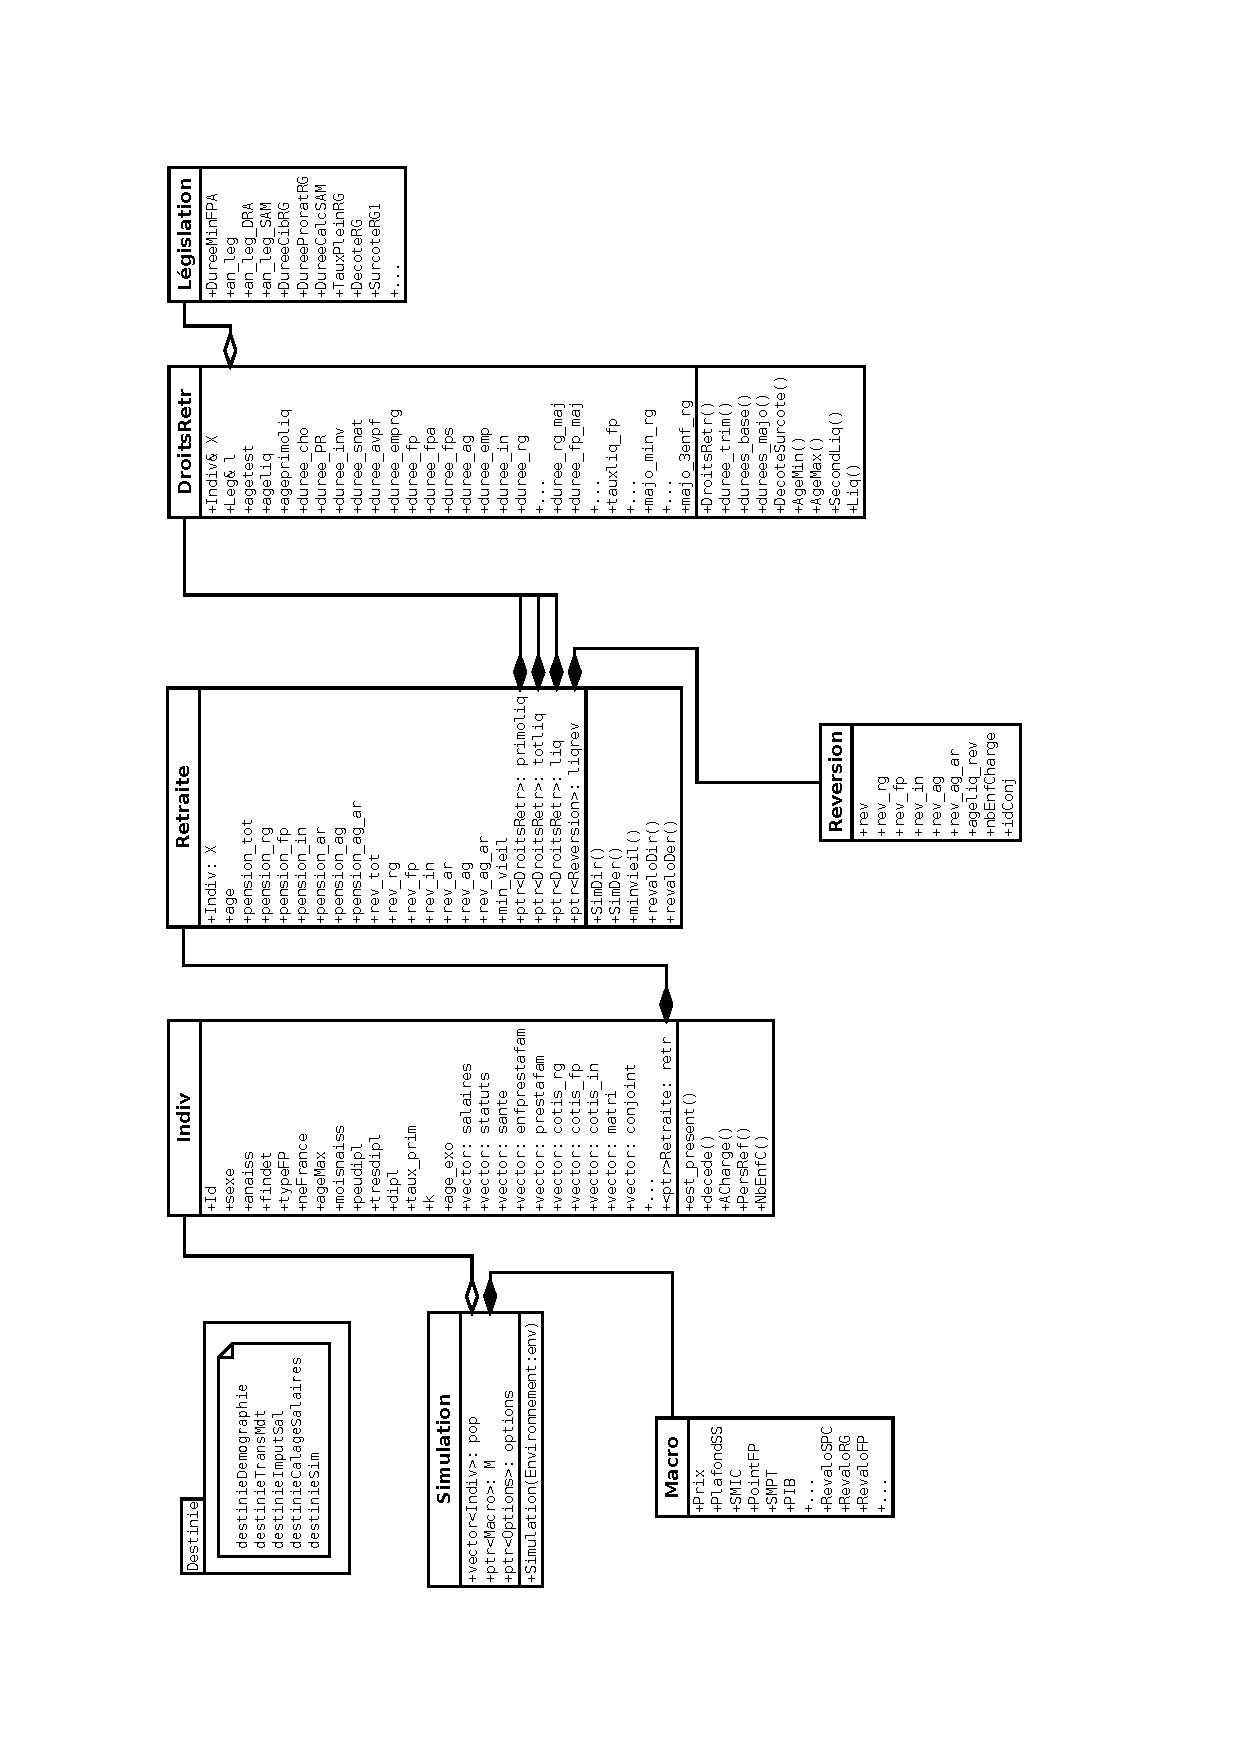
\includegraphics[scale=0.85,angle=270,origin=c]{Diagramme2.pdf}
\end{figure}
\end{landscape}

\subsection{Options et paramètres de simulation}
Un vaste choix d'options et de paramètres permet une simulation à la carte. Ce choix concerne les hypothèses démographiques, économiques et règlementaires.

\subsubsection{Hypothèses démographiques}
Les scénarios démographiques se distinguent par leurs variantes sur trois composantes que sont la natalité, la mortalité et le solde migratoire. Pour chaque composante, trois variantes existent : centrale (modalité \textit{Cent}), basse (modalité \textit{Bas}), haute (modalité \textit{Haut}). Il existe autant de scénarios que de croisements possibles entre ces variantes, soit 27. Les scénarios s'appuient sur les projections démographiques de l'Insee de 2016, couvrant la période 2013-2070.

\subsubsection{Hypothèses économiques}
Le cadre macroéconomique est défini selon deux axes : le scénario de chômage et de productivité. Trois scénarios de taux de chômage de long terme sont proposés : 4,5\%, 7\%, 10\%. Quant à la productivité, elle évolue selon quatre variantes de croissance tendancielle : 1,0\%, 1,3\%, 1,5\%, 1,8\%.

\subsubsection{Hypothèses règlementaires et autres}
Avant d'effectuer une simulation, certains autres paramètres doivent être renseignés dans l'objet \textit{options}. Il s'agit :
\begin{itemize}
\item de la dernière année de législation (variable \textit{anLeg})
\item du mode de comportement de liquidation\footnote{Bien que plusieurs modèles soient proposés, la plupart n'ont pas été expertisés depuis un certain temps. Le choix le plus prudent est celui du départ au taux plein (modalité "tp").}
\item du pas de test de liquidation entre l'âge d'ouverture des droits et l'âge d'annulation de la décote (variable \textit{pas1})
\item du pas de test de liquidation avant l'âge d'ouverture des droits et après l'âge d'annulation de la décote (variable \textit{pas2})
\item de l'horizon de projection (variable \textit{AN\_MAX})
\item du champ de la projection : France entière (modalité "FE") ou métropolitaine (modalité "FM")
\end{itemize}
D'autres options existent et sont détaillées dans \textbf{mettre lien vers partie sur les options de simulation}. Parmi celles-ci, toutes les options booléennes valent par défaut 0.

\subsection{Choix de Législation possibles}
La liquidation des droits se fait selon la législation en vigueur à une date choisie par l'utilisateur, stockée dans la variable \textit{anLeg} de l'objet \textit{options}. La législation est alors figée à celle prévalant à cette date.

\subsubsection{Réforme de 1993}

\begin{itemize}
\item	Concerne uniquement les salariés du secteur privé et les régimes alignés ;
\item Allongement progressif de la durée d'assurance requise pour accéder au taux plein (modification progressive pour les générations 1934-1943 à raison d'un trimestre supplémentaire par génération) ;
\item	Calcul du salaire de référence sur les 25 meilleures années au lieu de 10 (modification progressive pour les générations 1934-1947 à raison d'une année supplémentaire par génération) ;
\item	Les pensions et les salaires portés au compte sont indexés sur les prix, et non plus sur les salaires (principe déjà en vigueur depuis 1987) ;
\end{itemize}
\href{http://www.legislation.cnav.fr/textes/cr/cn/TLR-CR_CN_10393_30121993.htm#323}%
{Circulaire n°103/93 du 30 décembre 1993 Caisse nationale d'assurance vieillesse}
% Table generated by Excel2LaTeX from sheet 'Feuil2'
\begin{table}[h]
  \centering
  \caption{Détail par génération de la période transitoire 1993}
    \begin{tabular}{rrr}
    \toprule
    Année de  & Nombre d'années retenues & Trimestres d'assurance  \\
    naissance & pour le calcul du SAM    & pour obtenir le taux plein \\
    \midrule
    1933 et avant & 10    & 150 \\
    1934  & 11    & 151 \\
    1935  & 12    & 152 \\
    1936  & 13    & 153 \\
    1937  & 14    & 154 \\
    1938  & 15    & 155 \\
    1939  & 16    & 156 \\
    1940  & 17    & 157 \\
    1941  & 18    & 158 \\
    1942  & 19    & 159 \\
    1943  & 20    & 160 \\
    1944  & 21    & 160 \\
    1945  & 22    & 160 \\
    1946  & 23    & 160 \\
    1947  & 24    & 160 \\
    1948 et au-delà & 25    & 160 \\
    \bottomrule
    \end{tabular}%
  \label{tab:addlabel}%
\end{table}%


\subsubsection{Réforme de 2003}

\paragraph{Le régime général}

\begin{itemize}
   \item	Allongement progressif de la durée d'assurance requise pour accéder au taux plein à partir de la génération 1949 (passage de 160 
         trimestres à 164)
   \item	Allongement de la durée intervenant dans le coefficient de proratisation, censée à terme évoluer comme la durée cible d'assurance
   \item	Réduction de la décote à partir de la génération 1944, de 0,5 point par an pour atteindre 5\% par annuité manquante pour les 
         générations nées après 1952 (la décote n'est appliquée que si la liquidation a lieu avant 65 ans)
   \item	Surcote de 3\% par année supplémentaire travaillée après le 1er janvier 2004 ; la surcote a été renforcée par le plan « emploi des 
seniors » au printemps 2005
   \item	Modification du mode de calcul du minimum contributif
   \item	Possibilité de départ anticipé pour carrière longue : depuis le 1er janvier 2004, les assurés qui ont commencé à travailler très 
         jeune (avant 18 ans), et qui ont eu une longue carrière  peuvent partir à la retraite avant 60 ans (la condition de début de carrière est 
         un obstacle pour les assurés nés à partir de 1953 qui ont connu une scolarité obligatoire jusqu'à 16 ans).
\end{itemize}

% Table generated by Excel2LaTeX from sheet 'Feuil2'
\begin{table}[h]
  \centering
  \caption{Détail par génération de la période transitoire 2003}
    \begin{tabular}{rrrrr}
    \toprule
              &                   & Trimestres    &                       & Trimestres \\
              & Nombre d'années   & d'assurance   & Minoration du taux    & d'assurance   \\
    Année de  & retenues pour     & pour obtenir  & par nombre de         & maximum retenus        \\
    naissance & le calcul du SAM  & le taux plein & trimestre manquant    & pour le calcul RG      \\
    \midrule
    1933 et avant & 10    & 150   & \multicolumn{1}{r}{\multirow{11}[0]{*}{-1,2500}} & \multicolumn{1}{r}{\multirow{11}[0]{*}{150}} \\
    1934  & 11    & 151   & \multicolumn{1}{c}{} & \multicolumn{1}{c}{} \\
    1935  & 12    & 152   & \multicolumn{1}{c}{} & \multicolumn{1}{c}{} \\
    1936  & 13    & 153   & \multicolumn{1}{c}{} & \multicolumn{1}{c}{} \\
    1937  & 14    & 154   & \multicolumn{1}{c}{} & \multicolumn{1}{c}{} \\
    1938  & 15    & 155   & \multicolumn{1}{c}{} & \multicolumn{1}{c}{} \\
    1939  & 16    & 156   & \multicolumn{1}{c}{} & \multicolumn{1}{c}{} \\
    1940  & 17    & 157   & \multicolumn{1}{c}{} & \multicolumn{1}{c}{} \\
    1941  & 18    & 158   & \multicolumn{1}{c}{} & \multicolumn{1}{c}{} \\
    1942  & 19    & 159   & \multicolumn{1}{c}{} & \multicolumn{1}{c}{} \\
    1943  & 20    & \multicolumn{1}{r}{\multirow{6}[0]{*}{160}} & \multicolumn{1}{r}{} & \multicolumn{1}{c}{} \\
    1944  & 21    & \multicolumn{1}{c}{} & -1,1875 & 152 \\
    1945  & 22    & \multicolumn{1}{c}{} & -1,1250 & 154 \\
    1946  & 23    & \multicolumn{1}{c}{} & -1,0625 & 156 \\
    1947  & 24    & \multicolumn{1}{c}{} & -1,0000 & 158 \\
    1948  & \multicolumn{1}{r}{\multirow{5}[0]{*}{25}} & \multicolumn{1}{r}{} & -0,9375 & 160 \\
    1949  & \multicolumn{1}{c}{} & 161   & -0,8750 & 161 \\
    1950  & \multicolumn{1}{c}{} & 162   & -0,8125 & 162 \\
    1951  & \multicolumn{1}{c}{} & 163   & -0,7500 & 163 \\
    1952  & \multicolumn{1}{c}{} & 164   & -0,6875 & 164 \\
    \bottomrule
    \end{tabular}%
  \label{tab:addlabel}%
\end{table}%

\paragraph{Fonction publique}

\begin{itemize}
	\item	Augmentation de la durée d'assurance à partir de 2004 pour rejoindre celle requise dans le régime général et ensuite progresser en 
         parallèle à partir de 2006
	\item	Décote de 0,5 point par annuité manquante, augmentée de 0,5 point à chaque génération pour atteindre 5\% en 2015 (avec hausse 
         progressive de l'âge pivot à partir duquel la décote s'annule)
	\item	Surcote de 3\% par année supplémentaire travaillée, comme dans le secteur privé
	\item	Modification du mode de calcul du minimum garanti
	\item	Modification des droits familiaux et conjugaux
\end{itemize}



\subsubsection{Réforme de 2010}

\begin{itemize}
	\item  Relèvement progressif de \textbf{l'âge légal de départ} à 
la retraite pour atteindre \textbf{62 ans} en 2018. Cette évolution 
concerne tous les salariés, du public comme du privé ainsi 
que les régimes spéciaux, mais avec des calendriers de mise 
en œuvre différents,
	\item   L'âge à partir duquel il est permis à un assuré, 
n'ayant pas la durée de cotisation requise, de bénéficier 
tout de même d'une retraite à taux plein, passe 
progressivement de \textbf{65 à 67 ans},
	\item   Le dispositif des \textbf{"carrières longues"} est modifié, 
les salariés ayant commencé avant 18 ans peuvent partir à la 
retraite au plus tôt, sous réserve d'avoir la durée de 
cotisation requise pour leur génération, plus 2 ans.
	\item   Pour les salariés qui, du fait d'une situation 
d'usure professionnelle, ont une incapacité physique 
supérieure ou égale à 20\%, l'âge légal de départ à la 
retraite reste fixé à 60 ans et aucune décote ne leur est 
appliquée,
	\item   Les jeunes en chômage non indemnisé peuvent 
valider jusqu'à 6 trimestres (au lieu de 4).
	% \item    pour les femmes, l'indemnité journalière perçue 
% pendant le congé maternité entrera dans le salaire de 
% référence sur lequel sera calculée la pension de retraite,
	% \item    de nouvelles recettes financières sont instaurées, 
% comme la hausse de la tranche la plus élevée de l'impôt sur 
% le revenu (\pct{41} au lieu de \pct{40}), l'augmentation des 
% taxes sur les stock-options et les retraites-chapeaux, le 
% relèvement des prélèvements forfaitaires sur les revenus du 
% capital et des taxes sur les dividendes perçus par les 
% actionnaires,
	% \item    l'objectif assigné au fonds de réserve des 
% retraites est modifié : ses réserves (36,2 milliards en 2010)
 % seront, à partir de 2011, ponctionnées annuellement (2,1 
% milliards) au profit de la Caisse d'amortissement de la 
% dette sociale (Cades). 
\end{itemize}

\subsubsection{Accélération du calendrier fixé en 2010 suite au projet de loi de financement de la sécurité sociale pour 2012}
La loi du 21 décembre 2011 relative au financement de la sécurité sociale en 2012 prévoit une accélération de la réforme de 2010 : l'âge légal de départ et l'âge d'annulation de la décote passent à 62 et 67 ans respectivement, dès 2017 au lieu de 2018.

\subsubsection{Décret de juillet 2012: extension du dispositif carrières longues}

Le décret du 2 juillet 2012 étend le dispositif de départs anticipés pour carrière longues, à compter de novembre 2012, aux personnes qui ont commencé à travailler avant 20 ans, et en supprime la condition relative à la durée d'assurance totale (la condition relative à la durée d'assurance cotisée est maintenue mais aménagée).

\subsubsection{Réforme de 2013}
\begin{itemize}
   \item Augmentation de la durée de cotisation d'un trimestre tous les 3 ans à partir de la génération née en 1958 pour atteindre 43 ans pour la génération 1973.
   \item Les périodes d'apprentissage, la formation, le chômage et la maternité sont mieux pris en compte.
   \item Un trimestre est considéré comme validé dès que le salarié a cotisé 200 heures au smic. Ce seuil passe à 150 heures au bénéfice des personnes à temps très partiel, avec un plafond fixé à 1,5 smic.
   \item Pour les salariés du public comme du privé, les cotisations patronales et salariales sont augmentées de 0,15 point chacune dès le 1er janvier 2014, puis de 0,05 point en 2015, 2016 et 2017.
   \item Mise en place d'un compte pénibilité.
   \item Le bonus pour les parents de trois enfants est fiscalisé.
   \item La revalorisation des pensions est décalée de six mois chaque année.
   \item Mise en place de la Lura (Liquidation unique des régimes alignés) à compter du 1er juillet 2017. Pour les individus ayant été affiliés à au moins deux des trois régimes alignés (régime général, régime social des indépendants et MSA-salariés), et dont la liquidation intervient à partir du 1er juillet 2017, la pension est calculée de façon unifiée. Le salaire de référence est calculée sur la base des 25 meilleures années (tous régimes confondus), et la durée validée par année est bornée à quatre trimestres (par exemple, pour un individu ayant validé quatre trimestres au régime général et deux trimestres au RSI au cours d'une année, seuls quatre trimestres sont pris en compte dans la durée d'assurance). Le versement de la pension, dû au titre des droits ouverts dans les trois régimes alignés, est assuré par le dernier régime d’affiliation. Sur ce point, Destinie 2 s'écarte de la législation : la pension est proratisée en fonction des durées validées dans chaque régime et les proratas sont comptés à la charge des régimes concernés. Cet écart permet d'évaluer les dépenses effectivement engagées par les régimes.
\end{itemize}

\subsubsection{Accord national interprofessionnel relatif aux retraites complémentaires Agirc-Arrco du 30 octobre 2015}
\begin{itemize}
   \item En 2016, 2017 et 2018, indexation de la valeur du service des points Agirc et Arrco sur l'inflation moins un point.
   \item En 2016, 2017 et 2018, indexation de la valeur d'achat des point Agirc et Arrco sur l'évolution du SMPT augmentée de deux points.
   \item Extension de la cotisation AGFF sur la tranche B à la tranche C à compter du 1er janvier 2016.
   \item Pour les individus liquidant leur retraite de base au taux plein, application d'un coefficient de minoration de 10\% sur la pension complémentaire, et ce, pour une durée de trois ans dans la limité de l'âge d'annulation de la décote. Ce coefficient ne s'applique pas aux individus qui liquident un an au moins après avoir rempli les conditions du taux plein. Pour les individus exonérés de la CSG ou soumis à un taux réduit, le coefficient ne s'applique pas ou est réduit.
   \item Pour les individus remplissant les conditions du taux plein dans les régimes de base mais reportant leur liquidation de la retraite complémentaire d'au moins deux années, application, pour une durée d'un an, d'un coefficient majorant :
   \begin{itemize}
   \item de 10\% si la liquidation a lieu au moins deux ans après
   \item de 20\% si la liquidation a lieu au moins trois ans après
   \item de 30\% si la liquidation a lieu au moins quatre ans après
   \end{itemize}
\end{itemize}



